\documentclass{nordic}
\usepackage[utf8]{inputenc}
\usepackage{graphicx}
\usepackage{amsmath}
\usepackage[colorlinks=true,linkcolor=black,citecolor=black,urlcolor=black]{hyperref}
\usepackage{siunitx}
\usepackage{caption}
\usepackage{subcaption}
\pagenumbering{gobble}

\newcommand{\NSCM}{27}
\newcommand{\submissionyear}{2014}
\newcommand{\submissiondate}{September 26th 2014}
\newcommand{\submissionpage}{http://congress.cimne.upc.es/nscm-\NSCM/frontal}

\header{
  \NSCM th Nordic Seminar on Computational Mechanics\\
  NSCM-\NSCM\\
  A. Eriksson, A. Kulachenko, M. Mihaescu and G. Tibert (Eds.)\\
  \copyright KTH, Stockholm, \submissionyear
}

\title{SPLINE BASED MESH GENERATOR FOR WIND TURBINE BLADES}

\author{
  E. Fonn$^{*\dag}$,
  A. Rasheed$^\dag$,
  A. M. Kvarving$^\dag$ and
  T. Kvamsdal$^{+\dag}$
}

\heading{
  E. Fonn,
  A. Rasheed,
  A. M. Kvarving and
  T. Kvamsdal
}

\address{
  $^*$E-mail: \url{eivind.fonn@sintef.no} \and

  $^\dag$Applied Mathematics, SINTEF ICT\\
%  Strindvegen 4\\
%ss  7034 Trondheim, Norway\\
  Web page: \url{http://www.sintef.no} \and

  $^+$Department of Mathematical Sciences, NTNU\\ 
}

\keywords{Isogeometry, Mesh Generation, Wind Turbine Blades, Transfinite Interpolation}

\abstract{%
  This paper details the development of a block structured spline based mesh generator for wind
  turbine blades, developed to streamline the workflow from CAD modeling to simulation and analysis.
}

\begin{document}
\maketitle

\section{INTRODUCTION}
Mesh generation involving complex geometries, such as wind turbines, is highly
complicated. The problem is generally addressed using tetrahedral meshes, or
hybrid meshes with hexahedral elements close to the body and tetrahedral
elements elsewhere. The popularity of such mesh generators can be attributed to
their associated ease of use and relative automation, which comes at the cost of
numerical accuracy in the subsequent analysis. Added to this, such meshes can
generally not represent the true geometry. Since 2005, isogeometric analysis
which offers an integration of analysis and CAD geometry through the same basis
functions is catching up. The method offers demonstrably better accuracy, as
well as an exact geometric representation. This method has, since its inception,
been applied to solving problems from the domain of fluid and structural
mechanics. The availability of NURBS-based surface modeling software such as
Rhinoceros has made it possible to create complex geometries with relative ease,
but the lack of a volumetric spline-based mesh generator proves to be a
bottleneck.

This work presents an automatic block-structured spline-based mesh generator for
wind turbine blades. It has been developed initially for the NREL 5MW reference
blade, but with a modular approach that will allow it to handle other geometries
as well.

\section{INPUT SPECIFICATION}
The NREL 5MW reference blade\cite{Jonkman2009drw} is defined in terms of
cross-sectional data at 19 points along the blade axis from $\SI{2}{m}$ to
$\SI{62.9}{m}$. At each point is defined the airfoil shape, its chord length,
the aerodynamic center as well as the twist angle. The innermost airfoils (until
about $\SI{10}{m}$) are cylindrical, the middle (until about $\SI{40}{m}$) are
DU (Delft University) airfoils of various kinds, and the outermost are NACA64
airfoils. See \autoref{fig:airfoils:note}.

In order to be able to create an ``O''-mesh, we impose a modification to each
airfoil to create a rounded trailing edge. This edge is uniformly $\SI{1}{cm}$
in size across the entire blade, independent of chord length. Relative to the
chord length, this modification is between $\SI{0.22}{\percent}$ and
$\SI{1.4}{\percent}$. See \autoref{fig:airfoils:te}, where the effect has been
exaggerated by a factor of five.

\begin{figure}
  \centering
  \begin{subfigure}[b]{0.40\textwidth}
    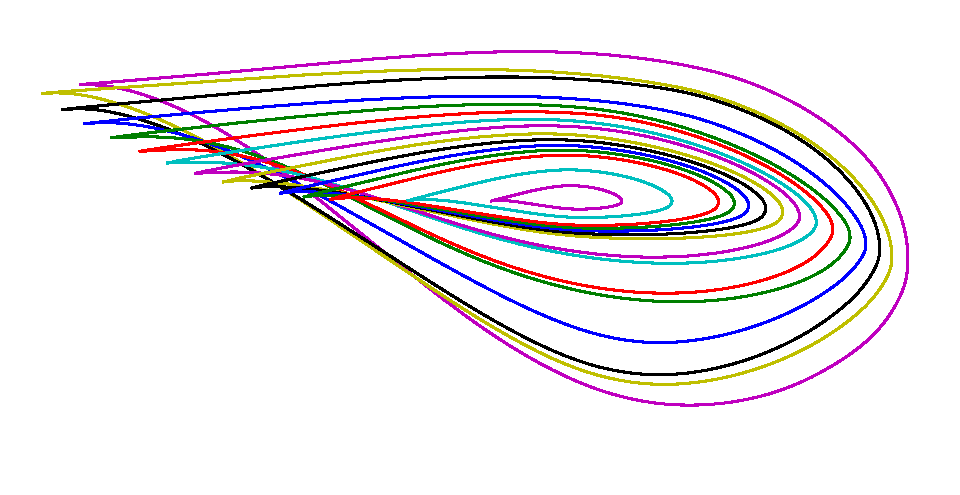
\includegraphics[width=\textwidth]{figs/airfoils-note}
    \caption{Sharp trailing edge}
    \label{fig:airfoils:note}
  \end{subfigure}
  \begin{subfigure}[b]{0.40\textwidth}
    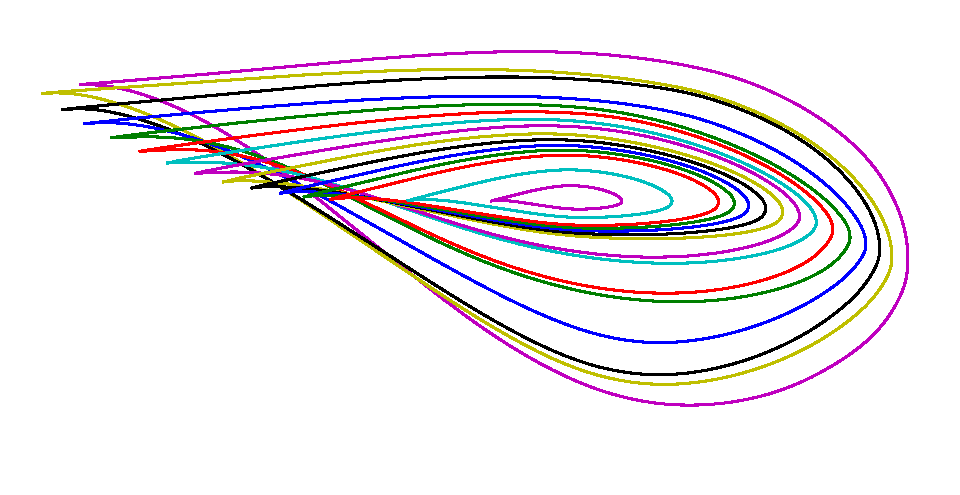
\includegraphics[width=\textwidth]{figs/airfoils-te}
    \caption{Exaggerated railing edge modification}
    \label{fig:airfoils:te}
  \end{subfigure}
  \caption{Airfoils for the NREL 5MW wind turbine blade.}
\end{figure}

\section{METHODOLOGY}

The whole procedure can be subdivided into two steps: solid modeling or blade construction and
volumetric mesh generation.  The mesh generation is performed using cubic splines everywhere, and the
spline order is then adjusted in the final step before output, to also allow the creation of linear
or quadratic models.

\subsection{BLADE CONSTRUCTION}

Simple cubic interpolation based on the cross sectional data can be used to form the complete blade
geometry from the hub at a radius of $\SI{2}{m}$ to the last cross section at $\SI{62.9}{m}$.  In
practice, the sharp transition from cylindrical cross sections to a narrow trailing edge will cause
the wall geometry to intersect with itself.  For this reason we employ a two-stage interpolation
process in this region.  An intermediate grid of sufficiently high resolution is formed with linear
interpolation, which can then be refined to the desired final resolution with a higher order
interpolator.

To close the tip we lift the central chord of the final cross section to a reasonably modest height
(around $\SI{20}{cm}$), and form cross section arcs at each node along the length of the
airfoil. $C^1$-continuity can be ensured by conforming to the known normal direction of the blade
geometry at the interface.  They are then lofted together and subdivided to form a 12-patch
structure.  See \autoref{fig:wingtip}.

\begin{figure}
  \centering
  \begin{subfigure}[b]{0.40\textwidth}
    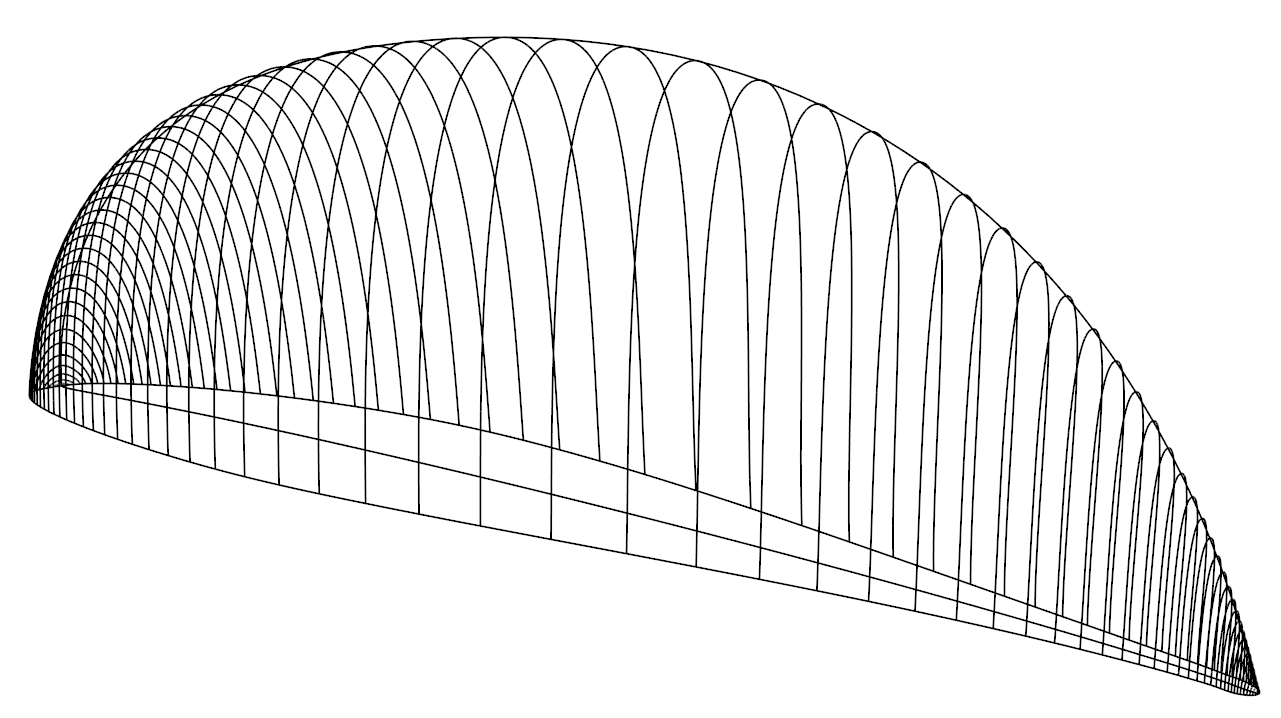
\includegraphics[width=\textwidth]{figs/wingtip-skeleton}
  \end{subfigure}
  \begin{subfigure}[b]{0.40\textwidth}
    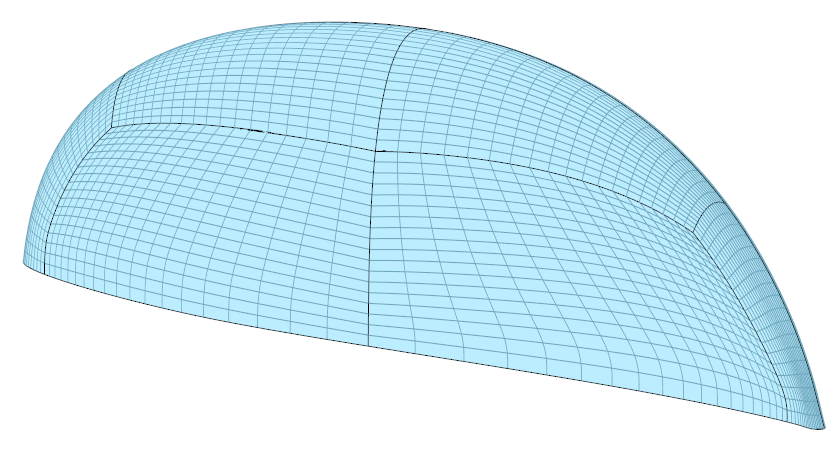
\includegraphics[width=\textwidth]{figs/wingtip-full}
  \end{subfigure}
  \caption{Closing the tip of the blade.}
  \label{fig:wingtip}
\end{figure}

\subsection{VOLUMETRIC MESH GENERATION}

At a given set of points along the blade, we wish to create a surrounding ``O''-mesh connecting the
airfoil to a circle with a given radius, centered at the aerodynamic center.  Transfinite
interpolation (TFI), also known as the Gordon Hall algorithm \cite{Gordon1973ccc}, is a useful method for
``filling in'' a surface between four curves or the volume between six surfaces.  However, it has
two crucial limitations:

\begin{itemize}
  \item The Jacobian is not guaranteed to be everywhere positive, which means gridlines might
    intersect.  This often happens for nonconvex domains.
  \item The gridlines close to the body are not guaranteed to be orthogonal, which is important for
    high Reynolds number CFD.
\end{itemize}

This causes problems near the trailing edge, as seen in \autoref{fig:tfi:bad}. To mitigate this, we
employ an algorithm that ``grows'' the mesh from the body outwards.  At each step, the gridlines are
projected some distance in the normal direction, after which a Laplacian smoothing is applied. The
final points are given by a weighted average with the ordinary TFI.  The weight, and the strength of
the smoothing, can be controlled by a coefficient that should be small in the boundary layer and
approach one relatively quickly away from it.  The final result can be observed in
\autoref{fig:tfi:good}.

\begin{figure}
  \centering
  \begin{subfigure}[b]{0.40\textwidth}
    \centering
    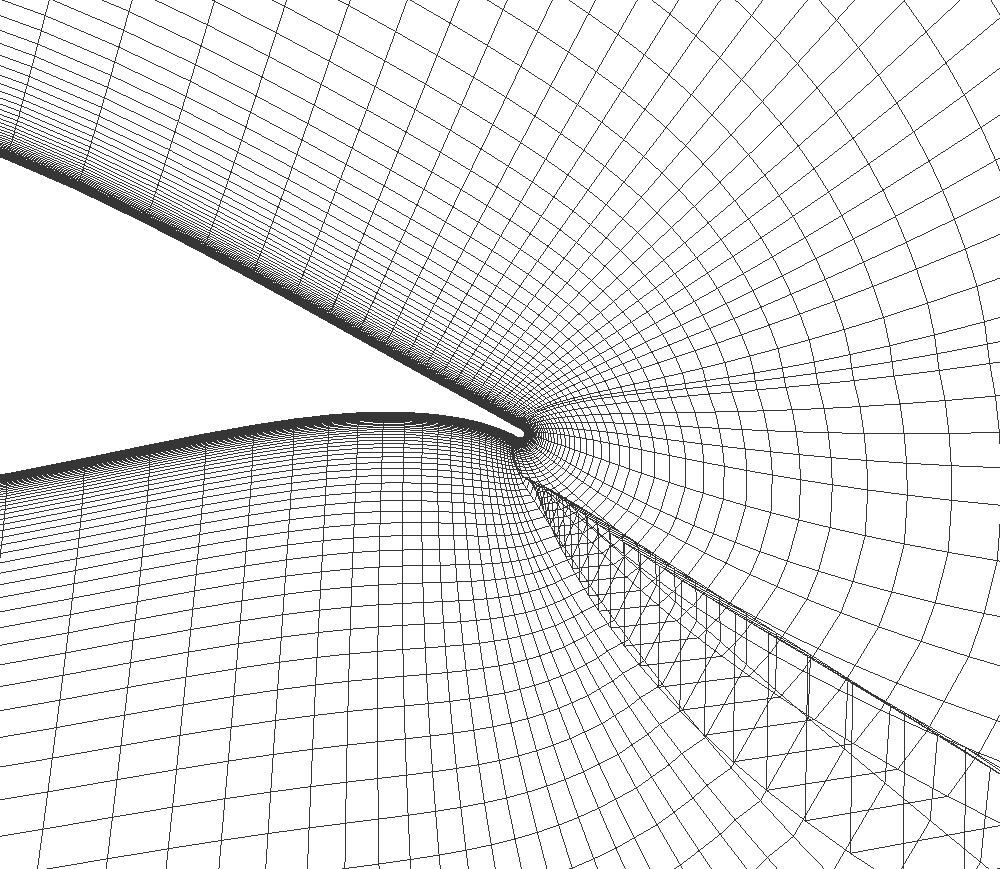
\includegraphics[width=0.75\textwidth]{figs/section12_zoom}
    \caption{Naive TFI}
    \label{fig:tfi:bad}
  \end{subfigure}
  \hspace{1cm}
  \begin{subfigure}[b]{0.40\textwidth}
    \centering
    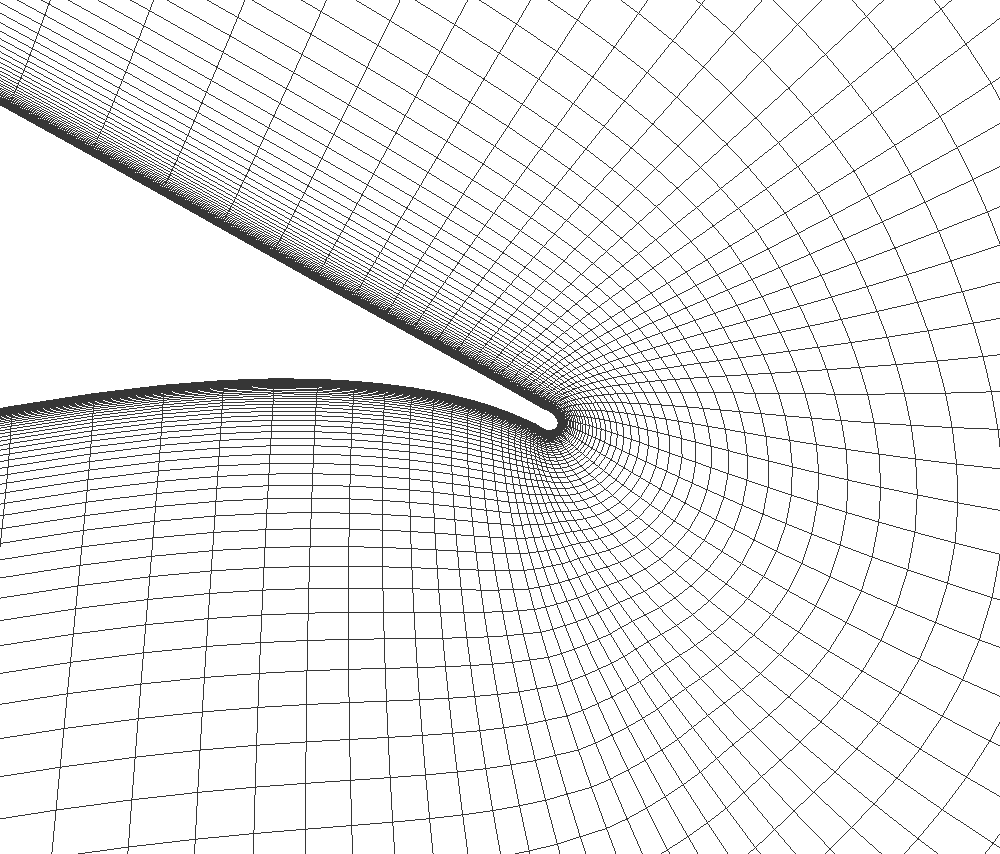
\includegraphics[width=0.75\textwidth]{figs/section12_smooth_zoom}
    \caption{Orthogonalized and smoothed TFI}
    \label{fig:tfi:good}
  \end{subfigure}
  \caption{Fixing the TFI algorithm}
\end{figure}

Precisely the same algorithm can be applied to the tip of the blade, but here we must deal with all
three dimensions simultaneously.  First, the tip is connected to the surrounding hemisphere with
interpolated curves, which are then filled in using two-dimensional TFI.  See \autoref{fig:tfi:tip}.

\begin{figure}[h!]
  \centering
  \begin{subfigure}[b]{0.40\textwidth}
    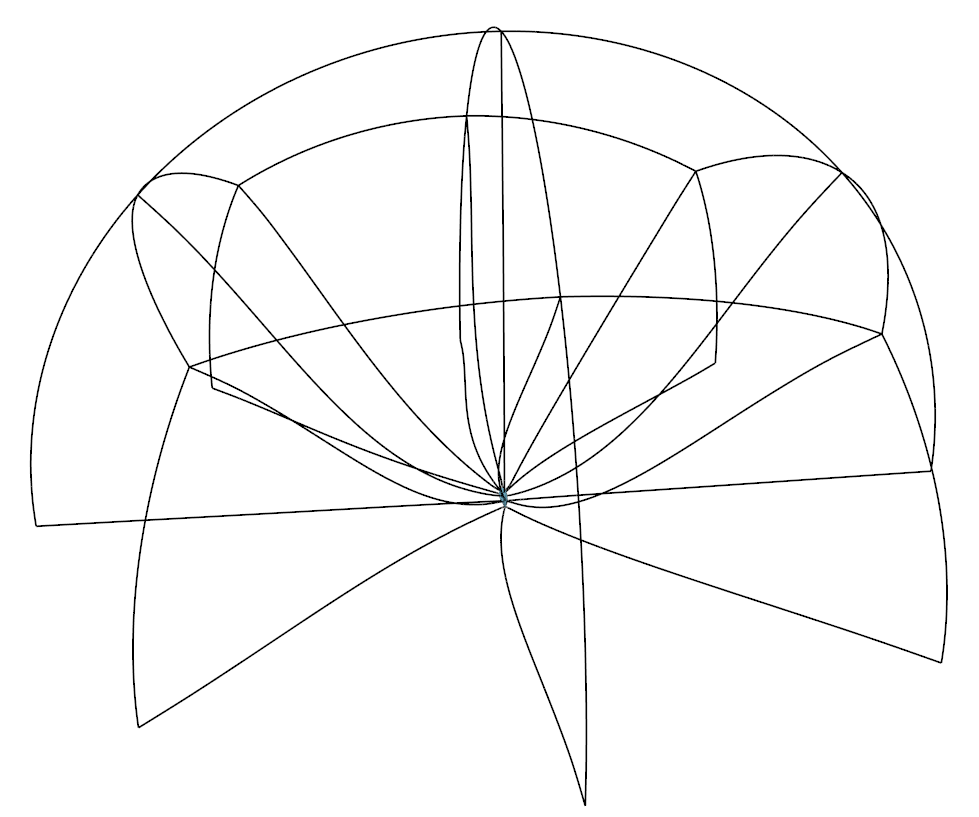
\includegraphics[width=\textwidth]{figs/wingtip-lines}
  \end{subfigure}
  \begin{subfigure}[b]{0.40\textwidth}
    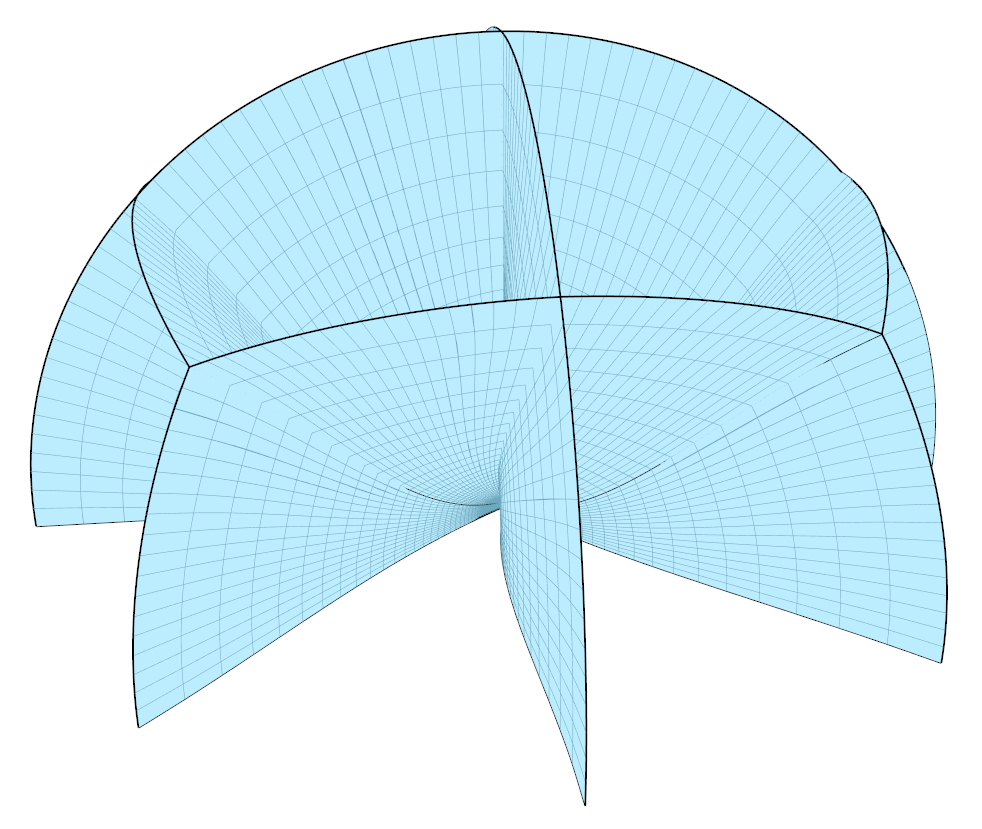
\includegraphics[width=\textwidth]{figs/wingtip-flower}
  \end{subfigure}
  \caption{Volumetric mesh for the tip}
  \label{fig:tfi:tip}
\end{figure}

After further subdivision (for purposes of parallelization), the final structure of the mesh might
look something like what is illustrated in \autoref{fig:full}.

\begin{figure}[h!]
  \centering
  \begin{subfigure}[b]{0.30\textwidth}
    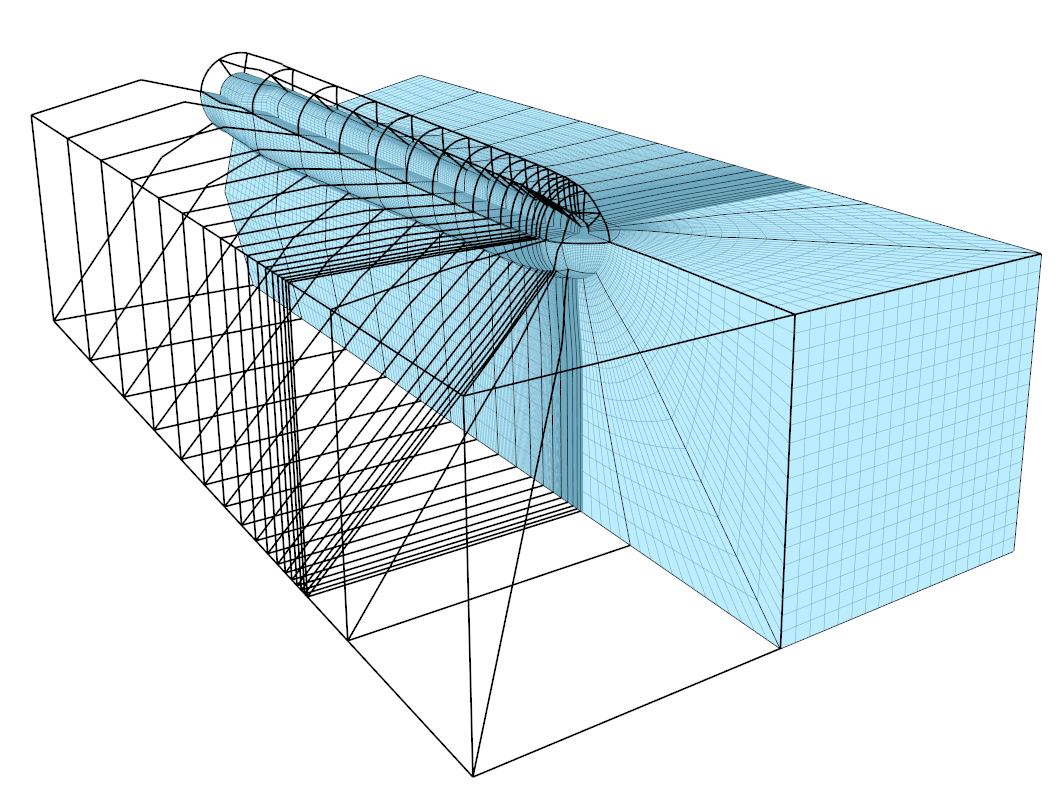
\includegraphics[width=\textwidth]{figs/structure-1}
  \end{subfigure}
  \begin{subfigure}[b]{0.30\textwidth}
    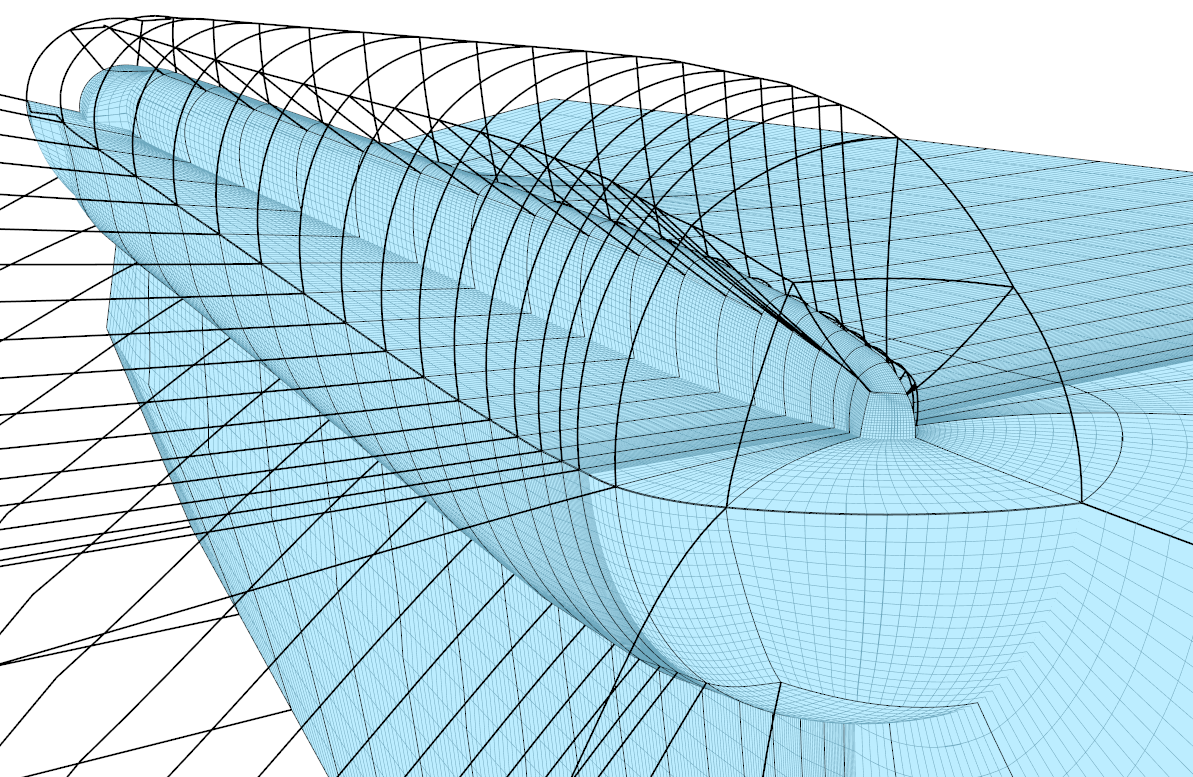
\includegraphics[width=\textwidth]{figs/structure-2}
  \end{subfigure}
  \begin{subfigure}[b]{0.30\textwidth}
    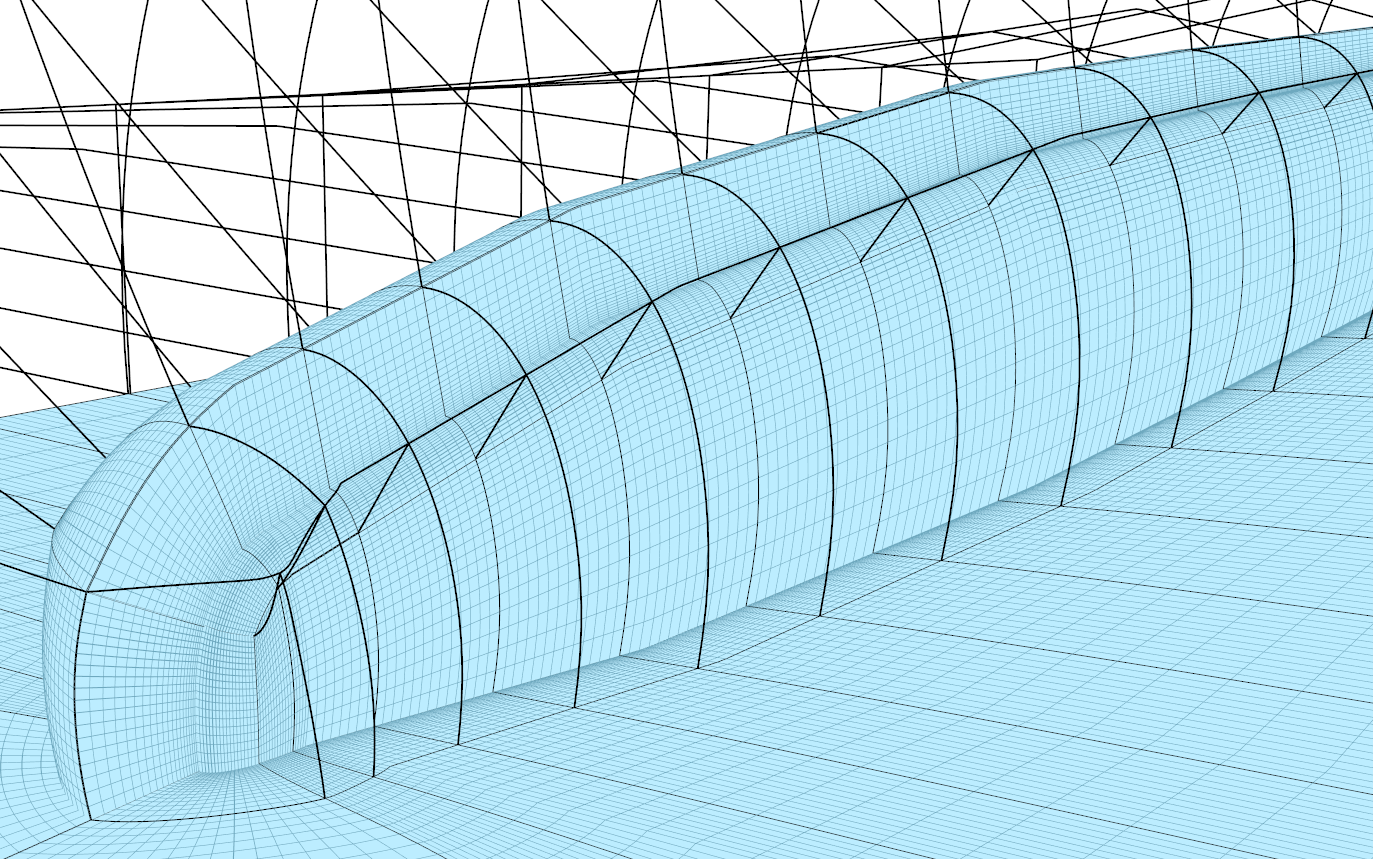
\includegraphics[width=\textwidth]{figs/structure-3}
  \end{subfigure}
  \caption{Full mesh structure}
  \label{fig:full}
\end{figure}

\section{CONCLUSION AND FUTURE WORK}

The mesh generator described in this work can be used to generate spline based meshes for
isogeometric analysis. The methodology ensures exact geometric representation and hexahedral elements
everywhere. The block structured meshing approach offers more flexibility in optimal load balancing
for high performance computing. Currently, the methodology applies to a single blade but work is in
progress to extend it to a full turbine containing any number of blades.

\section{ACKNOWLEDGEMENT}

The authors acknowledge the financial support from the Norwegian Research Council and the industrial
partners of the FSI-WT (216465/E20) (\url{http://www.fsi-wt.no}) and NOWITECH: Norwegian Research Centre
for Offshore Wind Technology (\url{http://www.nowitech.no}) projects.

\bibliography{common/references}
\bibliographystyle{naturemag}

\end{document}
